%!TEX TS-program = xelatex
\documentclass[]{friggeri-cv}
\usepackage{afterpage}
\usepackage{hyperref}
\usepackage{color}
\usepackage{xcolor}
\usepackage{smartdiagram}
\usepackage{fontspec}
% if you want to add fontawesome package
% you need to compile the tex file with LuaLaTeX
% References:
%   http://texdoc.net/texmf-dist/doc/latex/fontawesome/fontawesome.pdf
%   https://www.ctan.org/tex-archive/fonts/fontawesome?lang=en
%\usepackage{fontawesome}
\usepackage{metalogo}
\usepackage{dtklogos}
\usepackage[utf8]{inputenc}
\usepackage{tikz}
\usetikzlibrary{mindmap,shadows}
\hypersetup{
    pdftitle={},
    pdfauthor={},
    pdfsubject={},
    pdfkeywords={},
    colorlinks=false,           % no lik border color
    allbordercolors=white       % white border color for all
}
\smartdiagramset{
    bubble center node font = \footnotesize,
    bubble node font = \footnotesize,
    % specifies the minimum size of the bubble center node
    bubble center node size = 0.35cm,
    %  specifies the minimum size of the bubbleshttps://www.overleaf.com/project/5a69207d7ec8731a8321ca06
    bubble node size = 0.5cm,
    % specifies which is the distance among the bubble center node and the other bubbles
    distance center/other bubbles = 0.4cm,
    % sets the distance from the text to the border of the bubble center node
    distance text center bubble = 0.4cm,
    % set center bubble color
    bubble center node color = lightpink,
    % define the list of colors usable in the diagram
    set color list = {materialcyan, materiallime, materialamber, materialteal, materialindigo, materialgreen, orange, materialorange, green, lightgray},
    % sets the opacity at which the bubbles are shown
    bubble fill opacity = 0.6,
    % sets the opacity at which the bubble text is shown
    bubble text opacity = 0.8,
}

\addbibresource{bibliography.bib}
\RequirePackage{xcolor}
\definecolor{pblue}{HTML}{EE4466}

\begin{document}
\header{Jean-Romain} {Prévost}
      {Sr Software Engineer}
      
% Fake text to add separator      
\fcolorbox{white}{gray}{\parbox{\dimexpr\textwidth-2\fboxsep-2\fboxrule}{%
.....
}}

% In the aside, each new line forces a line break
\begin{aside}
    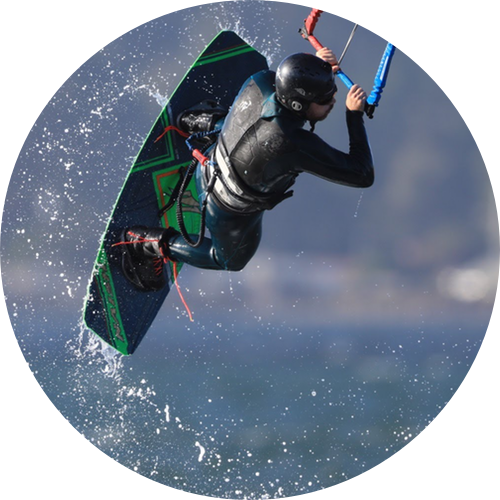
\includegraphics[scale=0.24]{img/cv-kite.png}
  ~
  ~
  ~
  \section{Info}
        411 Ashbury ave
        94530 El Cerrito
        (650)422-4814
        ~
        \href{mailto:jr@ailleurs.me}{\textbf{jr@ailleurs.me}}
        \href{https://www.linkedin.com/in/jeanromain/}{/in/jeanromain}
        \href{https://github.com/3on}{github.com/3on}
  ~
  ~
  ~
  ~
% use  \hspace{} or \vspace{} to change bubble size, if needed
  \section{Skills}
    ~
    \smartdiagram[bubble diagram]{
        \textbf{JavaScript},
        \textbf{React},
        \textbf{HTML5}\\\textbf{CSS3},
        \textbf{~Node.js~},
        \textbf{Python},
        \textbf{PHP},
        \textbf{Swift},
        \textbf{Git}
    }
\end{aside}
~
~
~
~
~
\section{Experience}
\begin{entrylist}
    \entry
    {08/18 - 01/20}
    {Sr Software Engineer}
    {Cruise}
    {As part of the Remote Assistance team, I contributed to a React web application that enabled remote control and monitoring of autonomous vehicles. I played a key role in improving tooling and test coverage, by adding support for tools such as: Enzyme, Storybook, Puppeteer. I spearheaded the rendering of the WebGL scene which relied on the internal library Worldview.\\}
    \entry
    {09/14 - 03/18}
    {Software Engineer}
    {Yelp}
    {On the website, I worked on the modernization of the web photos experience and the web homepage redesign projects. Both projects required a complete rewrite front-end and back-end. I mainly focused on the the front-end side of both projects. The homepage project also required code packaging as part of the micro-services transition, which I lead on the front-end.\\
    On the iOS application, I worked on improving various components of the business page: photo carousel header, search facet, bookmarks etc.
    Other contributions include mentoring (intern and new hire) and pushing code to production every other week.
    \\}
    \entry
    {07/13 - 09/14}
    {Software Engineer}
    {Montage Studio}
    {Montage Studio was a tool made in Montage.js to ease the creation of a Montage.js application. Montage.js is a rich JavaScript framework that borrows a lot of Cocoa's UI design patterns. I was part of the team making Montage Studio, which was entirely written in JavaScript (Node.js and Montage.js). I made various rich UI components such as a tree viewer or replicate OSX's context menus.\\}
    \entry
    {06/13 - 10/13}
    {Open Source Contributor}
    {VideoLAN}
    {In my spare time, I contributed to the open source project VLC. I submitted various patches for the iOS App. My most noticeable contribution is the little web application that runs on the phone that eases uploading content to the device using a built-in web server.\\}
    \entry
    {02/12 - 02/13}
    {Software Engineer Intern}
    {dotCloud (now Docker)}
    {I was part of a moonshot project, dotCloud JS. It was an open source library providing server-less data persistence. I worked on the library, documentation and marketing website. I was also a core contributor to dotCloud's web dashboard. It is was a single page application made in Backbone.js and Bootstrap. I worked on decreasing the learning curve for new users making boiler-plate apps and interactive walk-throughs. I used WebSockets and File API to bring the web UI closer to feature parity with the CLI tool.\\}
\end{entrylist}
  ~
 \pagebreak
  ~
\section{Education}
\begin{entrylist}
  \entry
    {2007 - 2012}
    {Master's Degree in Computer Science}
    {EPITA}
    {4 year engineering school focused on computer science. I majored in Web and Mobile technologies (MTI: Multimédia et Technologies de l’Information).\\}
  \entry
    {\phantom{2006 -} 2006}
    {JavaScript and PHP classes}
    {UCSD Extensions}
    {I completed two introduction night classes to PHP and JavaScript at UCSD while in high school.\\}
  \entry
    {2003 - 2007}
    {Baccalauréat}
    {Lycée Félix Faure}
    {Baccalauréat Scientifique SVT option européenne, mention AB.}
\end{entrylist}

\begin{aside}
  ~
  ~
  \section{Passions}
  ~
    \smartdiagram[bubble diagram]{
        \textbf{Kite-}\\\textbf{boarding},
        \textbf{Skiing},
        \textbf{Cooking},
        \textbf{Mountain}\\\textbf{biking},
        \textbf{Motor-}\\\textbf{cycling},
        \textbf{Cat}\\\textbf{hiking}
    }
    ~
\end{aside}

\end{document}
